% ----------------------------------------------------
% -------- BAYSIS - Selected as Jam Effector ---------
% ----------------------------------------------------
\subsection{BAYSIS - Selected as Jam Effector}
\label{analysis_processing_correlation_baysis_effector}
The correlation matrix table for the congestion-accident \textit{Jam Effector} dataset (see \cref{table:appendix_correlation_matrix_matched_cramers}) is visual presented in \cref{img:correlation_matrix_selected_effector_cramers} showing the the correlation of each variable combination. When visual analyzing \cref{img:correlation_matrix_matched_cramers} and checking the guidelines for a strong correlation in reference to the applied coefficient (identifiable with \cref{table:appendix_coefficient_matrix_matched}) we get a list of strongly correlated variable combinations (see \cref{tbl:correlation_list_baysis_effector})

\noindent
\begin{table}[h!]
	\centering
	\begin{tabular}{c|l}  
		Category & Strong \\
		\\[-1em]
		\hline
		\\[-1em]
		Strasse & TMax, TAvg, SMax, SAvg, Cov, TLHGV \\ 
 		Kat & TMax, TAvg, SAvg \\ 
 		%Typ & \\
 		%Betei & \\
 		UArt1 & SAvg \\
 		UArt2 & SMax \\
 		%AUrs1 & \\
 		%AUrs2 & \\
 		AufHi & TMax, TAvg \\
 		%Alkoh & \\
 		%Char1 & \\
 		%Char2 & \\
 		%Bes1 & \\
 		%Lich1 & \\
 		%Lich2 & \\
 		%Zust1 & \\
 		%Zust2 & \\
 		%Fstf & \\
 		WoTag & TAvg, SMax, Cov, TLHGV \\
 		%FeiTag & \\
 		Month & TMax, TAvg, SMax, SAvg, Cov, TLHGV \\
	\end{tabular}
    \caption{List of incident variables and their strong correlated congestion variable from the congestion-accident matched data which are classified as \textit{Jam Effector}}
	\label{tbl:correlation_list_baysis_effector}
\end{table}

% \newgeometry{left=1.5cm,right=1cm}
% 	\pagestyle{empty}
% 	\begin{figure}[ht]
% 		\centering
% 		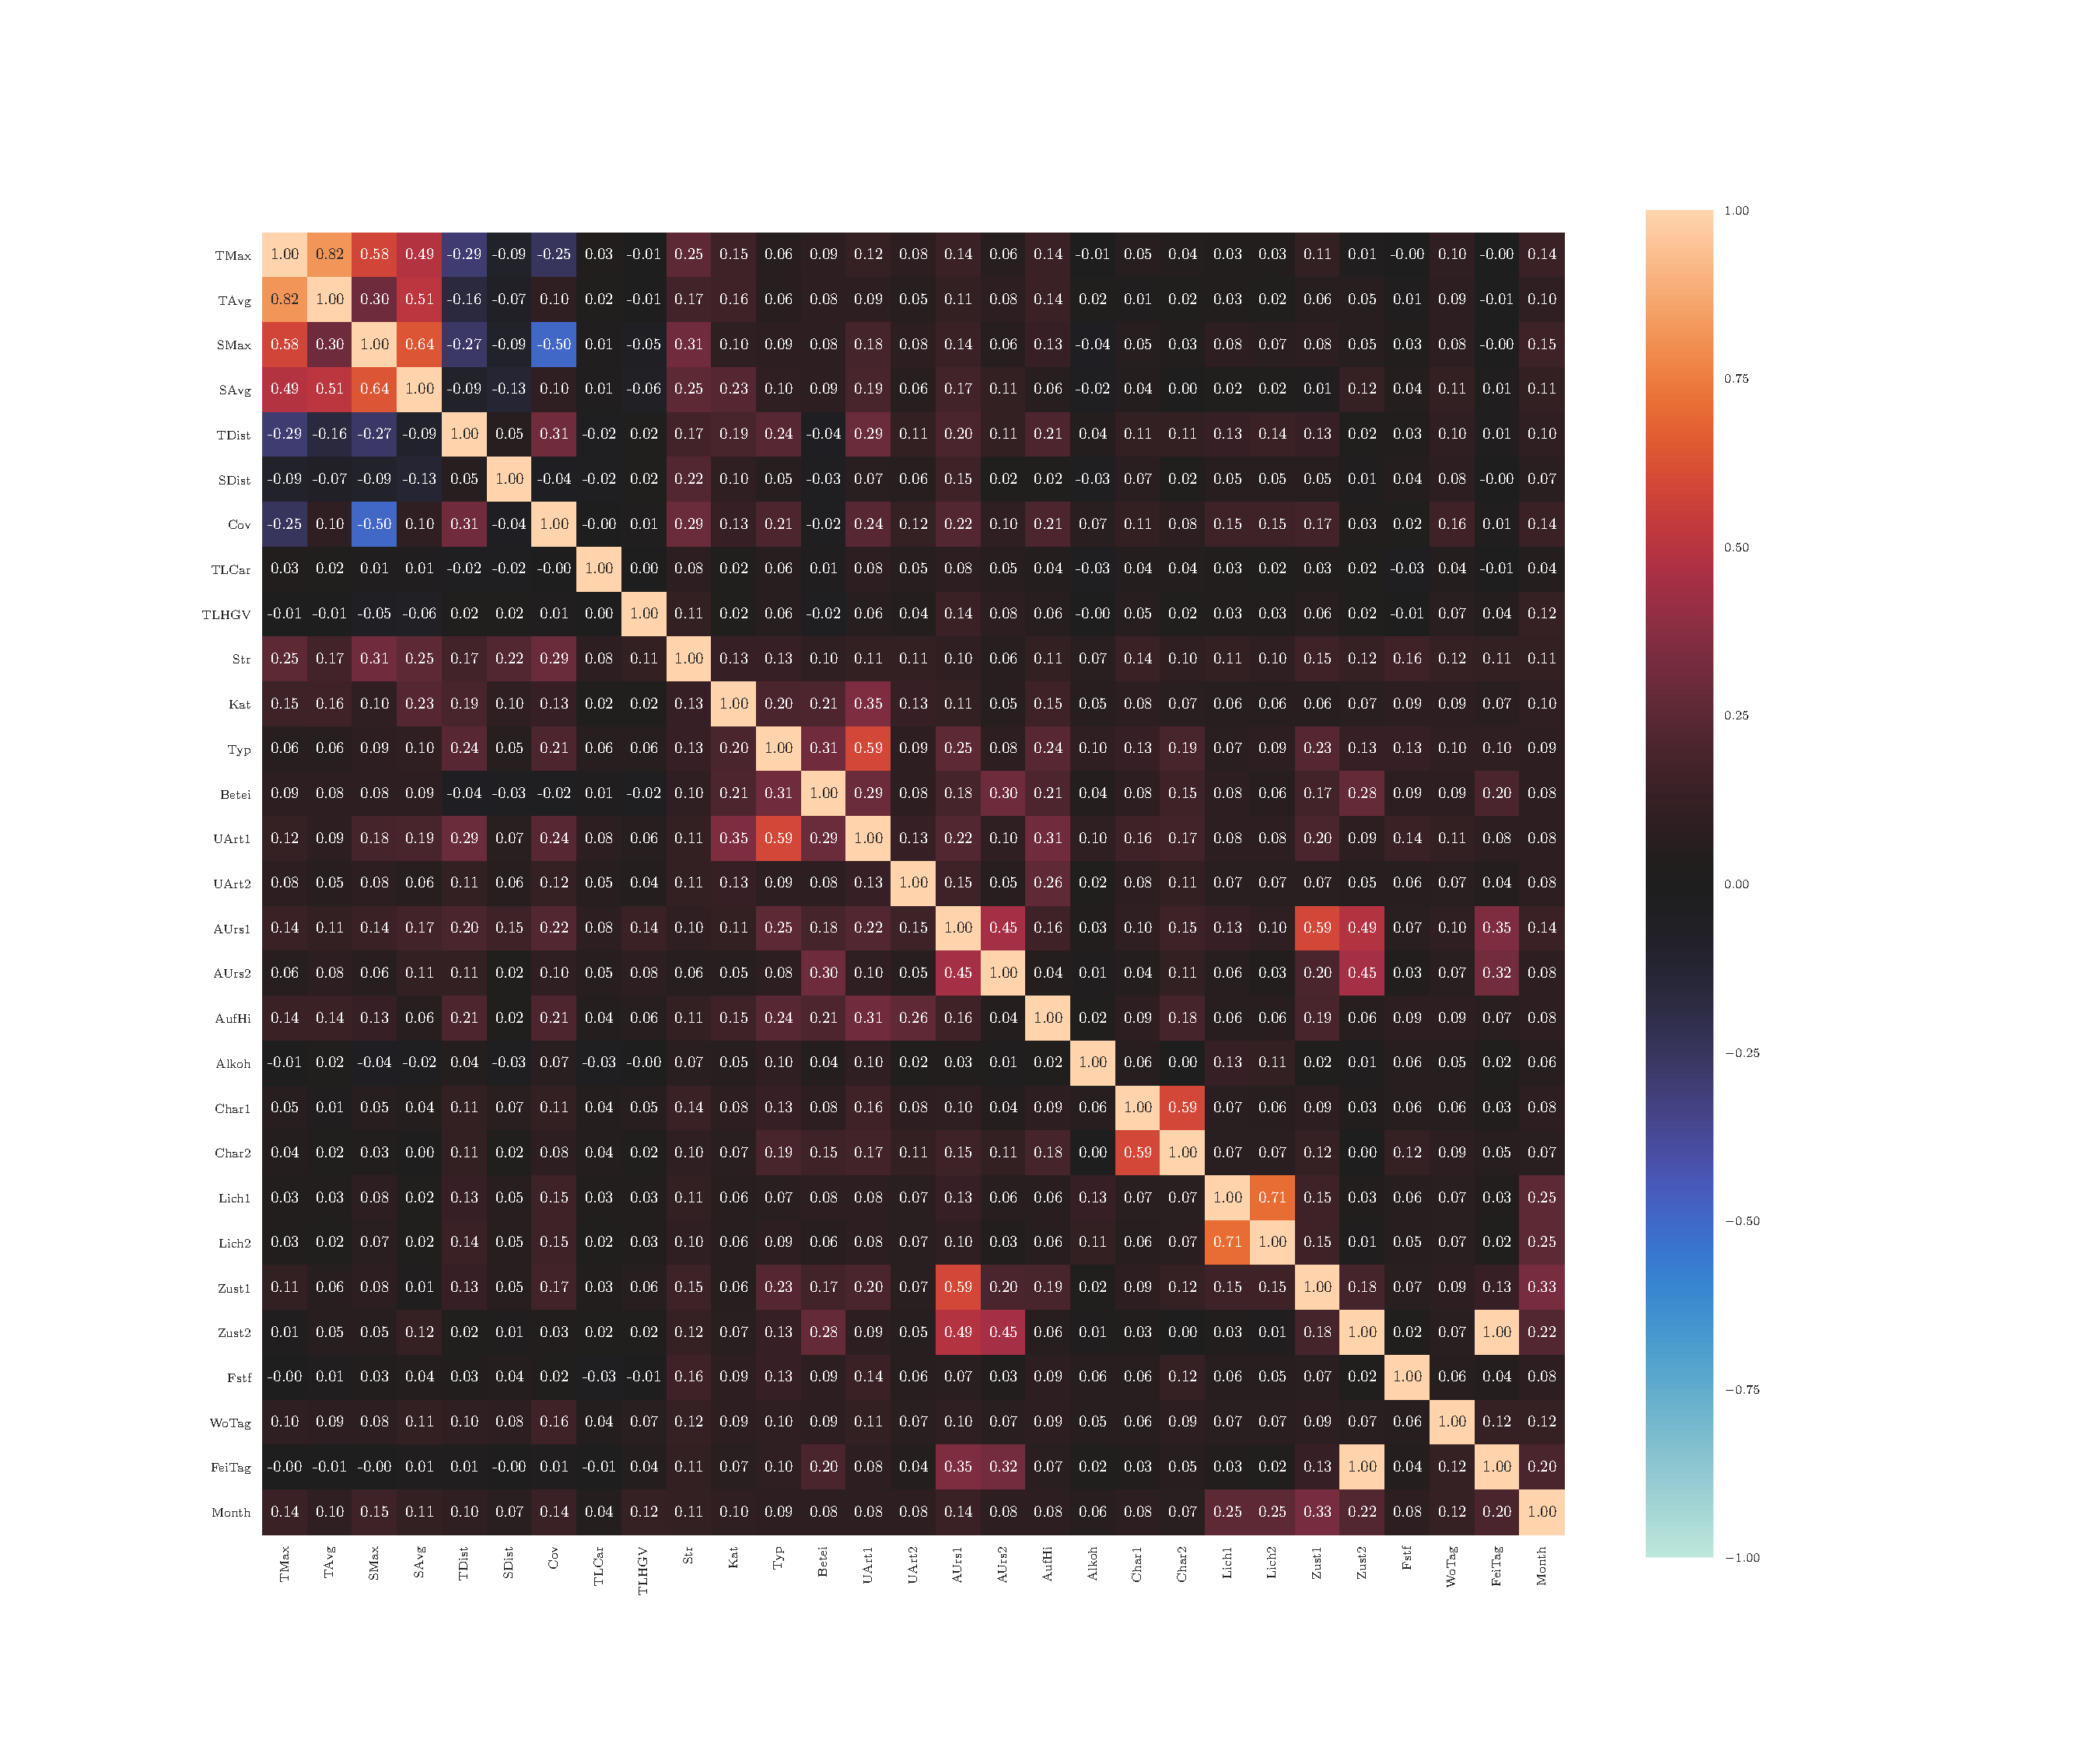
\includegraphics[scale=0.52, trim=3cm 2cm 0cm 0cm]{../CorrAnalysis/data/BAYSIS/02_matched/plots/baysis_matched_corr_cramers}
% 		\caption{Correlation matrix for BAYSIS matched data, with $V$, $\eta$, $\tau$, $r_{pq}$, $r$}
% 		\label{img:correlation_matrix_matched_cramers}
% 	\end{figure}
% \restoregeometry
\begin{figure}[!ht]
	\centering
	\makebox[\textwidth][c]{%
		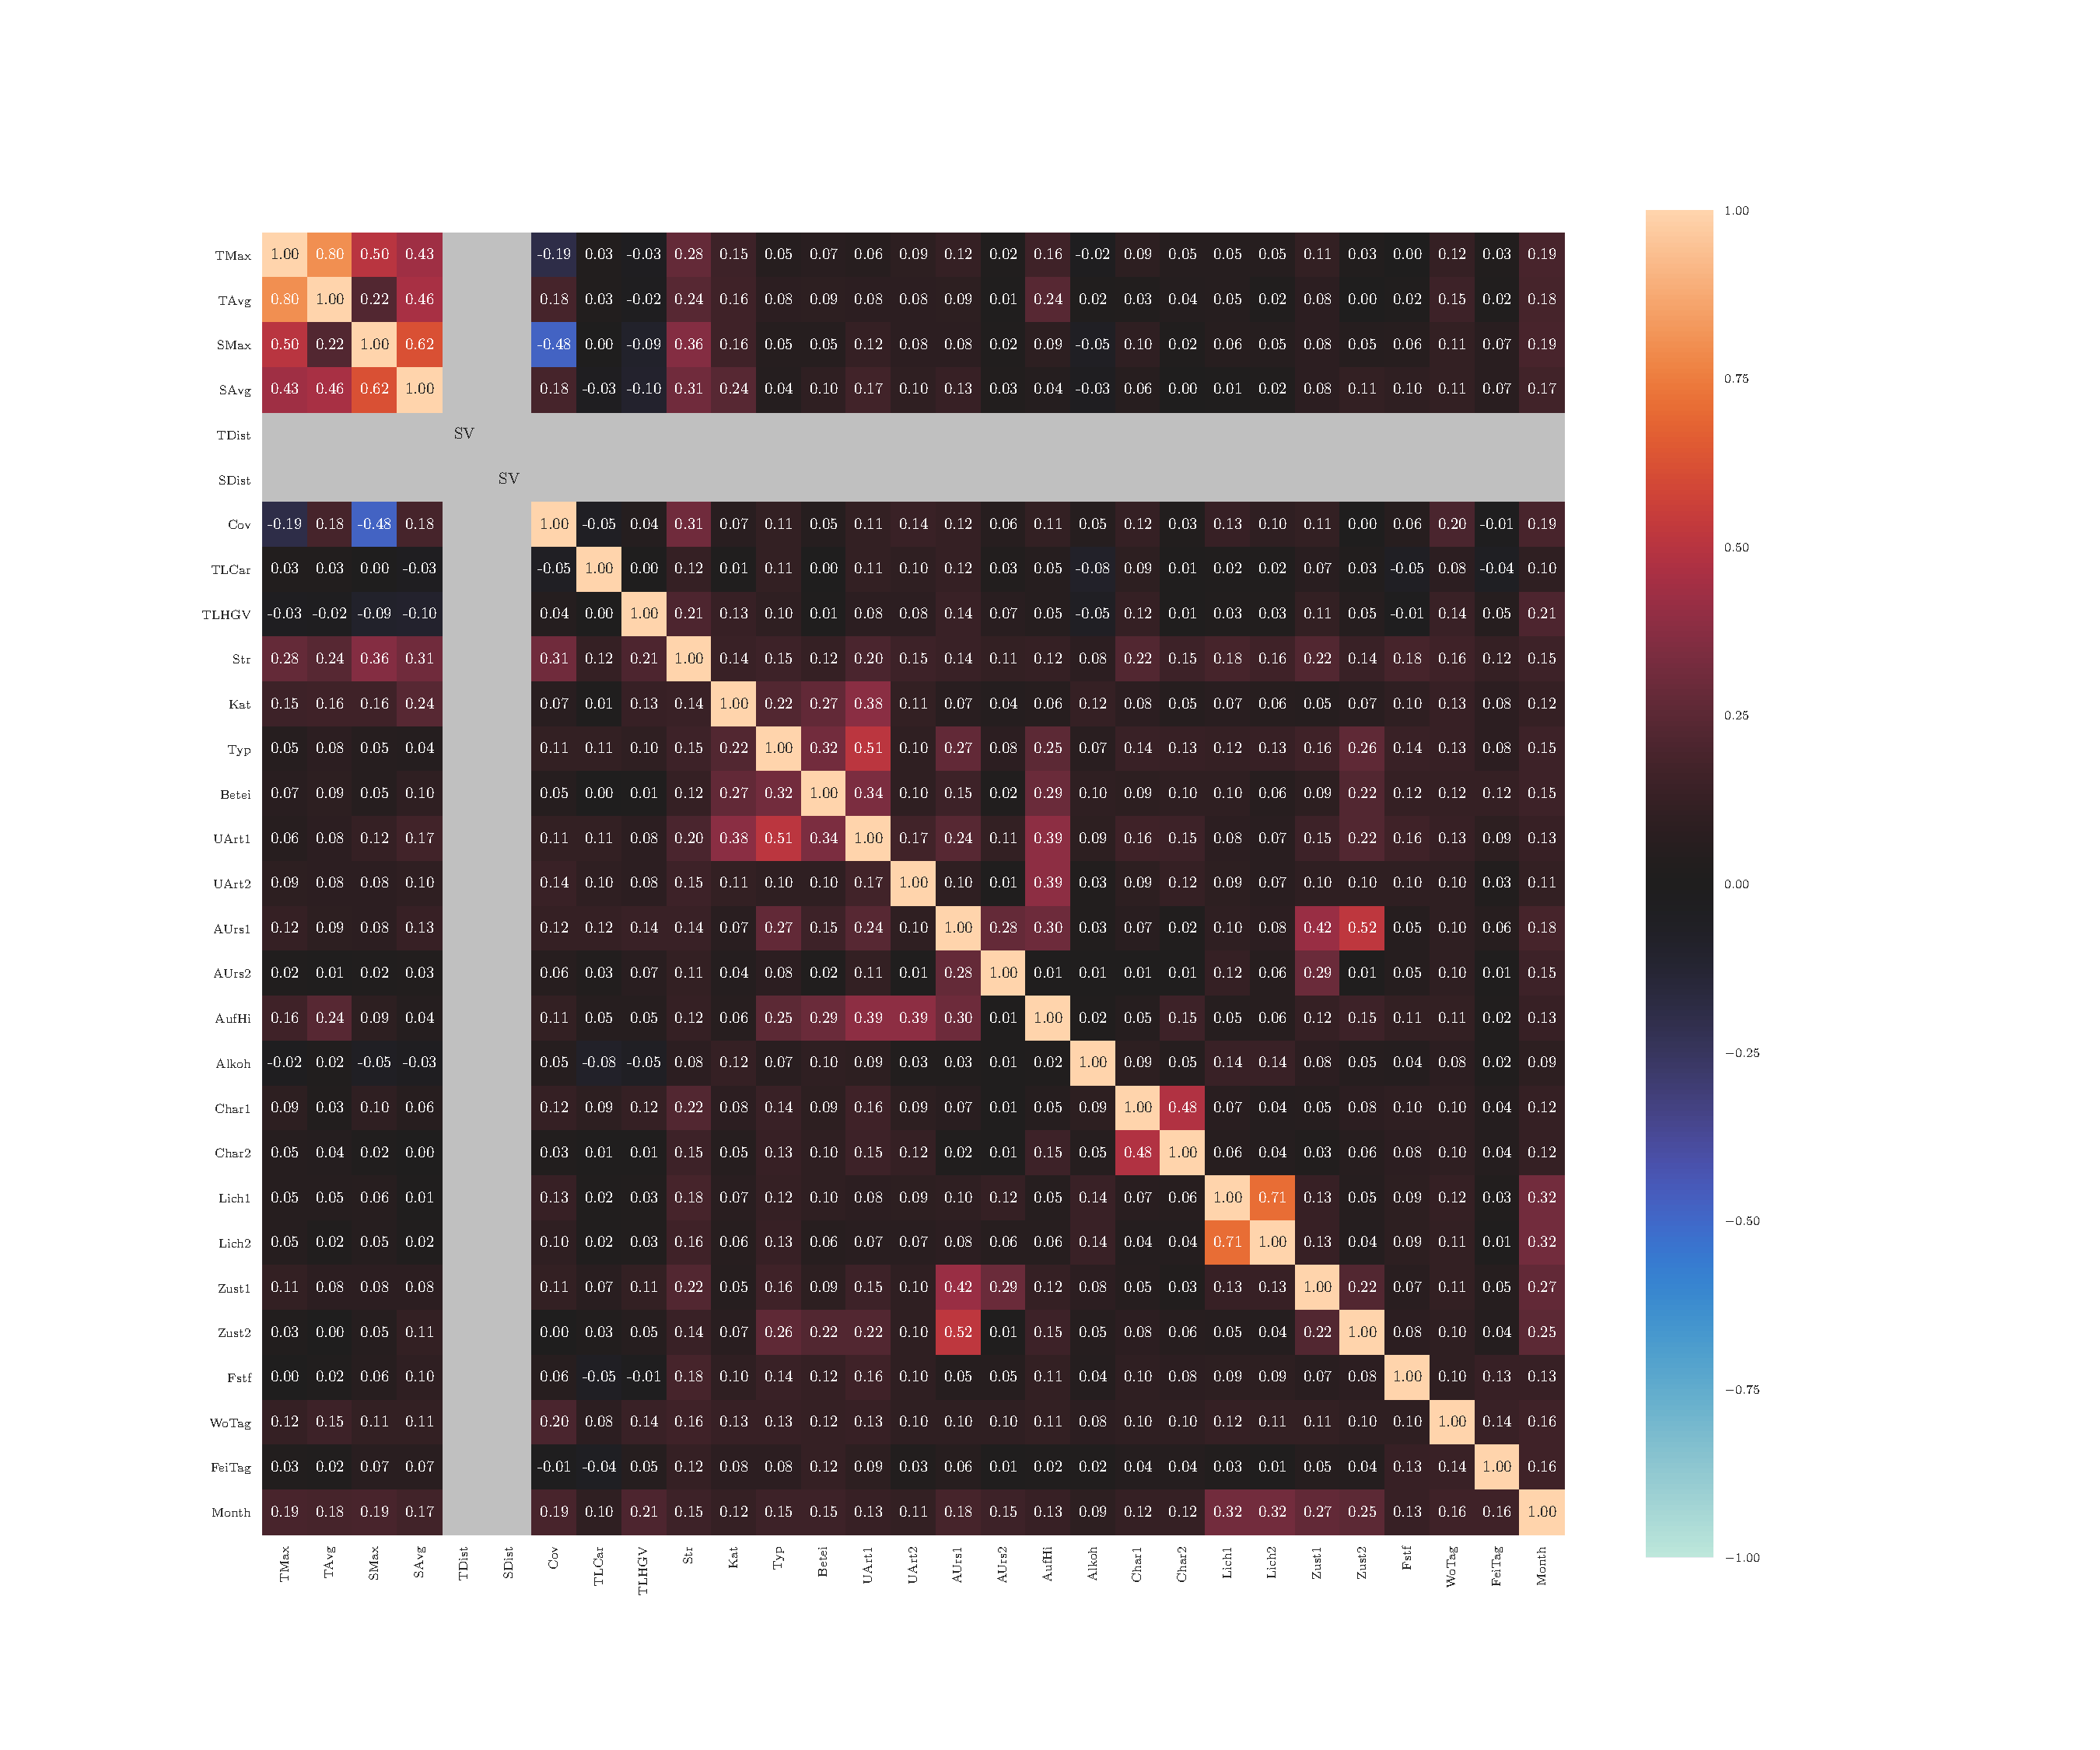
\includegraphics[width=1.4\textwidth, trim=0cm 2.5cm 6cm 3cm]{CorrAnalysis/data/BAYSIS/03_selected_02_duringJam/plots/baysis_selected_corr_cramers}%
	}
	\caption{Correlation matrix for congestion-accident matched data classified as \textit{Jam Effector}, with $V$, $\eta$, $\tau$, $r_{pq}$, $r$}
	\label{img:correlation_matrix_selected_effector_cramers}
\end{figure}

\large
\centerline{\textbf{Strasse}}
\normalsize

\paragraph{Maximal Temporal Extent}
Kruskal-Wallis chi-squared = 255.99, df = 199, p-value = 0.003967

\begin{table}[ht]
	\small
	\centering
	\begin{tabular}{rrrrrrrrrrrrrr}
		\toprule
		& A3 & A6 & A9 & A70 & A99 & A93 & A94 & A7 & A73 & A96 & A995 & A92 & A95 \\ 
		\midrule
		1 & 1.00 &  &  &  &  &  &  &  &  &  &  &  &  \\ 
		2 & 0.23 & 1.00 &  &  &  &  &  &  &  &  &  &  &  \\ 
		3 & 1.00 & 1.00 & 1.00 &  &  &  &  &  &  &  &  &  &  \\ 
		4 & 0.28 & 1.00 & 1.00 & 1.00 &  &  &  &  &  &  &  &  &  \\ 
		5 & 1.00 & 1.00 & 1.00 & 1.00 & 1.00 &  &  &  &  &  &  &  &  \\ 
		6 & 0.01 & 1.00 & 0.06 & 1.00 & 0.28 & 1.00 &  &  &  &  &  &  &  \\ 
		7 & 0.87 & 1.00 & 1.00 & 1.00 & 1.00 & 1.00 & 1.00 &  &  &  &  &  &  \\ 
		8 & 0.00 & 1.00 & 0.00 & 1.00 & 0.23 & 1.00 & 1.00 & 1.00 &  &  &  &  &  \\ 
		9 & 0.00 & 1.00 & 0.34 & 1.00 & 1.00 & 1.00 & 1.00 & 1.00 & 1.00 &  &  &  &  \\ 
		10 & 1.00 & 1.00 & 1.00 & 1.00 & 1.00 & 1.00 & 1.00 & 1.00 & 1.00 & 1.00 &  &  &  \\ 
		11 & 0.01 & 1.00 & 0.24 & 1.00 & 1.00 & 1.00 & 1.00 & 1.00 & 1.00 & 1.00 & 1.00 &  &  \\ 
		12 & 1.00 & 1.00 & 1.00 & 1.00 & 1.00 & 1.00 & 1.00 & 1.00 & 1.00 & 1.00 & 1.00 & 1.00 &  \\ 
		13 & 1.00 & 1.00 & 1.00 & 1.00 & 1.00 & 1.00 & 1.00 & 1.00 & 1.00 & 1.00 & 1.00 & 1.00 &  \\ 
		\bottomrule
	  \end{tabular}
    \caption{Pairwise Wilcoxon $T$-test for \textit{AUrs1} and \textit{Coverage}}
    \label{tbl:wilcoxon_baysis_effector_AUrs1_Cov}
\end{table}
\todo{Explain}
\begin{table}[ht]
	\small
	\centering
	\begin{tabular}{rrrrrrrrrrrrrr}
		\toprule
		& vars & n & mean & sd & median & trimmed & mad & min & max & range & skew & kurtosis & se \\ 
		\midrule
	X1 & 1.00 & 278.00 & 311.57 & 227.68 & 252.00 & 285.13 & 200.15 & 18.00 & 1257.00 & 1239.00 & 1.08 & 0.93 & 13.66 \\ 
		X11 & 1.00 & 37.00 & 236.59 & 183.03 & 207.00 & 216.48 & 195.70 & 18.00 & 705.00 & 687.00 & 0.92 & 0.09 & 30.09 \\ 
		X12 & 1.00 & 192.00 & 243.45 & 178.97 & 201.00 & 219.06 & 142.33 & 15.00 & 1194.00 & 1179.00 & 1.70 & 4.54 & 12.92 \\ 
		X13 & 1.00 & 7.00 & 151.29 & 106.95 & 138.00 & 151.29 & 44.48 & 24.00 & 369.00 & 345.00 & 0.94 & -0.25 & 40.42 \\ 
		X14 & 1.00 & 63.00 & 212.57 & 140.78 & 195.00 & 192.94 & 115.64 & 21.00 & 681.00 & 660.00 & 1.35 & 1.94 & 17.74 \\ 
		X15 & 1.00 & 12.00 & 212.00 & 187.74 & 130.50 & 191.70 & 124.54 & 39.00 & 588.00 & 549.00 & 0.74 & -1.13 & 54.19 \\ 
		X16 & 1.00 & 14.00 & 109.71 & 56.07 & 97.50 & 103.75 & 53.37 & 42.00 & 249.00 & 207.00 & 0.93 & 0.14 & 14.99 \\ 
		X17 & 1.00 & 35.00 & 254.66 & 306.21 & 168.00 & 186.31 & 133.43 & 42.00 & 1341.00 & 1299.00 & 2.53 & 5.99 & 51.76 \\ 
		X18 & 1.00 & 52.00 & 157.21 & 179.42 & 130.50 & 132.57 & 66.72 & 18.00 & 1323.00 & 1305.00 & 5.25 & 31.35 & 24.88 \\ 
		X19 & 1.00 & 41.00 & 155.85 & 84.33 & 144.00 & 144.82 & 53.37 & 30.00 & 381.00 & 351.00 & 1.23 & 1.19 & 13.17 \\ 
		X110 & 1.00 & 1.00 & 9.00 &  & 9.00 & 9.00 & 0.00 & 9.00 & 9.00 & 0.00 &  &  &  \\ 
		X111 & 1.00 & 21.00 & 134.71 & 82.25 & 138.00 & 128.29 & 75.61 & 18.00 & 354.00 & 336.00 & 0.74 & 0.24 & 17.95 \\ 
		X112 & 1.00 & 1.00 & 99.00 &  & 99.00 & 99.00 & 0.00 & 99.00 & 99.00 & 0.00 &  &  &  \\ 
		X113 & 1.00 & 1.00 & 99.00 &  & 99.00 & 99.00 & 0.00 & 99.00 & 99.00 & 0.00 &  &  &  \\ 
		\bottomrule
	  \end{tabular}
    \caption{Group descriptives of \textit{AUrs1} and \textit{Coverage}}
    \label{tbl:descriptives_baysis_effector_AUrs1_Cov}
	%\vspace{-8mm}
\end{table}

\paragraph{Average Temporal Extent}
Kruskal-Wallis chi-squared = 291.56, df = 210, p-value = 0.0001665

\begin{table}[ht]
	\small
	\centering
	\begin{tabular}{rrrrrrrrrrrrrr}
		\hline
	   & 0 & 1 & 2 & 3 & 4 & 5 & 6 & 7 & 8 & 9 & 10 & 11 & 12 \\ 
		\hline
	  1 & 1.00 &  &  &  &  &  &  &  &  &  &  &  &  \\ 
		2 & 1.00 & 1.00 &  &  &  &  &  &  &  &  &  &  &  \\ 
		3 & 1.00 & 1.00 & 1.00 &  &  &  &  &  &  &  &  &  &  \\ 
		4 & 0.01 & 1.00 & 1.00 & 1.00 &  &  &  &  &  &  &  &  &  \\ 
		5 & 1.00 & 1.00 & 1.00 & 1.00 & 1.00 &  &  &  &  &  &  &  &  \\ 
		6 & 0.08 & 1.00 & 0.53 & 1.00 & 1.00 & 1.00 &  &  &  &  &  &  &  \\ 
		7 & 1.00 & 1.00 & 1.00 & 1.00 & 1.00 & 1.00 & 0.61 &  &  &  &  &  &  \\ 
		8 & 0.00 & 1.00 & 0.00 & 1.00 & 1.00 & 1.00 & 1.00 & 0.02 &  &  &  &  &  \\ 
		9 & 1.00 & 1.00 & 1.00 & 1.00 & 1.00 & 1.00 & 1.00 & 1.00 & 0.87 &  &  &  &  \\ 
		10 & 1.00 & 1.00 & 1.00 & 1.00 & 1.00 & 1.00 & 1.00 & 1.00 & 1.00 & 1.00 &  &  &  \\ 
		11 & 0.90 & 1.00 & 1.00 & 1.00 & 1.00 & 1.00 & 1.00 & 1.00 & 1.00 & 1.00 & 1.00 &  &  \\ 
		12 & 1.00 & 1.00 & 1.00 & 1.00 & 1.00 & 1.00 & 1.00 & 1.00 & 1.00 & 1.00 & 1.00 & 1.00 &  \\ 
		13 & 1.00 & 1.00 & 1.00 & 1.00 & 1.00 & 1.00 & 1.00 & 1.00 & 1.00 & 1.00 & 1.00 & 1.00 & 1.00 \\ 
		 \hline
	  \end{tabular}
    \caption{Pairwise Wilcoxon $T$-test for \textit{AUrs1} and \textit{Coverage}}
    \label{tbl:wilcoxon_baysis_effector_AUrs1_Cov}
\end{table}
\todo{Explain}
\begin{table}[ht]
	\small
	\centering
	\begin{tabular}{rrrrrrrrrrrrrr}
		\hline
	   & vars & n & mean & sd & median & trimmed & mad & min & max & range & skew & kurtosis & se \\ 
		\hline
	  X1 & 1.00 & 278.00 & 103.46 & 85.35 & 83.00 & 91.06 & 55.60 & 7.00 & 703.00 & 696.00 & 2.58 & 11.45 & 5.12 \\ 
		X11 & 1.00 & 37.00 & 82.43 & 74.19 & 70.00 & 72.23 & 66.72 & 3.00 & 301.00 & 298.00 & 1.39 & 1.67 & 12.20 \\ 
		X12 & 1.00 & 192.00 & 91.31 & 74.64 & 75.00 & 79.71 & 49.67 & 5.00 & 575.00 & 570.00 & 2.27 & 8.79 & 5.39 \\ 
		X13 & 1.00 & 7.00 & 57.43 & 23.24 & 53.00 & 57.43 & 11.86 & 19.00 & 91.00 & 72.00 & -0.12 & -1.20 & 8.78 \\ 
		X14 & 1.00 & 63.00 & 65.73 & 47.32 & 52.00 & 59.06 & 26.69 & 4.00 & 295.00 & 291.00 & 2.25 & 7.35 & 5.96 \\ 
		X15 & 1.00 & 12.00 & 104.83 & 112.03 & 55.00 & 90.80 & 55.60 & 7.00 & 343.00 & 336.00 & 0.98 & -0.59 & 32.34 \\ 
		X16 & 1.00 & 14.00 & 45.93 & 25.54 & 43.00 & 43.92 & 30.39 & 14.00 & 102.00 & 88.00 & 0.66 & -0.68 & 6.82 \\ 
		X17 & 1.00 & 35.00 & 143.74 & 255.78 & 76.00 & 85.59 & 41.51 & 15.00 & 1326.00 & 1311.00 & 3.59 & 12.48 & 43.23 \\ 
		X18 & 1.00 & 52.00 & 47.63 & 29.09 & 44.00 & 44.29 & 20.76 & 6.00 & 154.00 & 148.00 & 1.28 & 1.92 & 4.03 \\ 
		X19 & 1.00 & 41.00 & 74.39 & 54.53 & 70.00 & 66.09 & 41.51 & 6.00 & 247.00 & 241.00 & 1.53 & 2.71 & 8.52 \\ 
		X110 & 1.00 & 1.00 & 9.00 &  & 9.00 & 9.00 & 0.00 & 9.00 & 9.00 & 0.00 &  &  &  \\ 
		X111 & 1.00 & 21.00 & 64.52 & 48.86 & 56.00 & 57.53 & 34.10 & 8.00 & 235.00 & 227.00 & 1.92 & 4.39 & 10.66 \\ 
		X112 & 1.00 & 1.00 & 50.00 &  & 50.00 & 50.00 & 0.00 & 50.00 & 50.00 & 0.00 &  &  &  \\ 
		X113 & 1.00 & 1.00 & 82.00 &  & 82.00 & 82.00 & 0.00 & 82.00 & 82.00 & 0.00 &  &  &  \\ 
		 \hline
	  \end{tabular}
    \caption{Group descriptives of \textit{AUrs1} and \textit{Coverage}}
    \label{tbl:descriptives_baysis_effector_AUrs1_Cov}
	%\vspace{-8mm}
\end{table}

\paragraph{Maximal Spatial Extent}
Kruskal-Wallis chi-squared = 752.33, df = 642, p-value = 0.001658

\begin{table}[ht]
	\small
	\centering
	\begin{tabular}{rrrrrrrrrrrrrr}
		\hline
	   & 0 & 1 & 2 & 3 & 4 & 5 & 6 & 7 & 8 & 9 & 10 & 11 & 12 \\ 
		\hline
	  1 & 1.00 &  &  &  &  &  &  &  &  &  &  &  &  \\ 
		2 & 0.00 & 1.00 &  &  &  &  &  &  &  &  &  &  &  \\ 
		3 & 0.92 & 1.00 & 1.00 &  &  &  &  &  &  &  &  &  &  \\ 
		4 & 1.00 & 1.00 & 1.00 & 1.00 &  &  &  &  &  &  &  &  &  \\ 
		5 & 0.05 & 0.13 & 1.00 & 1.00 & 1.00 &  &  &  &  &  &  &  &  \\ 
		6 & 0.01 & 0.03 & 0.41 & 1.00 & 0.24 & 1.00 &  &  &  &  &  &  &  \\ 
		7 & 0.03 & 0.65 & 1.00 & 1.00 & 1.00 & 1.00 & 1.00 &  &  &  &  &  &  \\ 
		8 & 0.00 & 0.00 & 0.00 & 1.00 & 0.00 & 1.00 & 1.00 & 0.93 &  &  &  &  &  \\ 
		9 & 0.04 & 1.00 & 1.00 & 1.00 & 1.00 & 1.00 & 1.00 & 1.00 & 0.18 &  &  &  &  \\ 
		10 & 1.00 & 1.00 & 1.00 & 1.00 & 1.00 & 1.00 & 1.00 & 1.00 & 1.00 & 1.00 &  &  &  \\ 
		11 & 0.00 & 0.00 & 0.04 & 1.00 & 0.04 & 1.00 & 1.00 & 1.00 & 1.00 & 1.00 & 1.00 &  &  \\ 
		12 & 1.00 & 1.00 & 1.00 & 1.00 & 1.00 & 1.00 & 1.00 & 1.00 & 1.00 & 1.00 & 1.00 & 1.00 &  \\ 
		13 & 1.00 & 1.00 & 1.00 & 1.00 & 1.00 & 1.00 & 1.00 & 1.00 & 1.00 & 1.00 & 1.00 & 1.00 & 1.00 \\ 
		 \hline
	  \end{tabular}
    \caption{Pairwise Wilcoxon $T$-test for \textit{AUrs1} and \textit{Coverage}}
    \label{tbl:wilcoxon_baysis_effector_AUrs1_Cov}
\end{table}
\todo{Explain}
\begin{table}[ht]
	\small
	\centering
	\begin{tabular}{rrrrrrrrrrrrrr}
		\hline
	   & vars & n & mean & sd & median & trimmed & mad & min & max & range & skew & kurtosis & se \\ 
		\hline
	  X1 & 1.00 & 278.00 & 24884.31 & 35913.14 & 15931.50 & 17906.50 & 11393.04 & 1566.00 & 219082.00 & 217516.00 & 4.10 & 17.21 & 2153.93 \\ 
		X11 & 1.00 & 37.00 & 16711.43 & 9518.81 & 14449.00 & 15820.94 & 8762.17 & 2655.00 & 40033.00 & 37378.00 & 0.86 & 0.08 & 1564.88 \\ 
		X12 & 1.00 & 192.00 & 13271.42 & 8473.71 & 11654.50 & 12297.11 & 8042.36 & 1315.00 & 49765.00 & 48450.00 & 1.21 & 2.03 & 611.54 \\ 
		X13 & 1.00 & 7.00 & 8698.57 & 2612.81 & 8969.00 & 8698.57 & 2865.87 & 3852.00 & 11096.00 & 7244.00 & -0.70 & -1.06 & 987.55 \\ 
		X14 & 1.00 & 63.00 & 17558.70 & 12223.42 & 14698.00 & 16701.86 & 12565.03 & 2351.00 & 48278.00 & 45927.00 & 0.58 & -0.87 & 1540.01 \\ 
		X15 & 1.00 & 12.00 & 8158.42 & 4473.23 & 7461.50 & 7808.30 & 3728.00 & 2896.00 & 16922.00 & 14026.00 & 0.69 & -0.77 & 1291.31 \\ 
		X16 & 1.00 & 14.00 & 7277.64 & 4218.45 & 6947.00 & 7094.25 & 4762.11 & 1206.00 & 15550.00 & 14344.00 & 0.17 & -1.03 & 1127.43 \\ 
		X17 & 1.00 & 35.00 & 11825.00 & 8885.99 & 9506.00 & 10484.55 & 6068.28 & 3041.00 & 43244.00 & 40203.00 & 1.62 & 2.72 & 1502.01 \\ 
		X18 & 1.00 & 52.00 & 7964.98 & 5995.59 & 6559.50 & 6953.33 & 3349.93 & 1036.00 & 33764.00 & 32728.00 & 2.07 & 5.27 & 831.44 \\ 
		X19 & 1.00 & 41.00 & 11825.98 & 6911.19 & 9676.00 & 11222.03 & 7924.50 & 2006.00 & 27965.00 & 25959.00 & 0.61 & -0.46 & 1079.35 \\ 
		X110 & 1.00 & 1.00 & 1772.00 &  & 1772.00 & 1772.00 & 0.00 & 1772.00 & 1772.00 & 0.00 &  &  &  \\ 
		X111 & 1.00 & 21.00 & 7255.76 & 3637.71 & 7364.00 & 7107.24 & 4601.99 & 1176.00 & 13522.00 & 12346.00 & 0.32 & -1.10 & 793.81 \\ 
		X112 & 1.00 & 1.00 & 4636.00 &  & 4636.00 & 4636.00 & 0.00 & 4636.00 & 4636.00 & 0.00 &  &  &  \\ 
		X113 & 1.00 & 1.00 & 1925.00 &  & 1925.00 & 1925.00 & 0.00 & 1925.00 & 1925.00 & 0.00 &  &  &  \\ 
		 \hline
	  \end{tabular}
    \caption{Group descriptives of \textit{AUrs1} and \textit{Coverage}}
    \label{tbl:descriptives_baysis_effector_AUrs1_Cov}
	%\vspace{-8mm}
\end{table}
\paragraph{Average Spatial Extent}
Kruskal-Wallis chi-squared = 704.4, df = 647, p-value = 0.05831

\paragraph{Coverage}
Kruskal-Wallis chi-squared = 127.9, df = 81, p-value = 0.0006961

\begin{table}[ht]
	\small
	\centering
	\begin{tabular}{rrrrrrrrrrrrrr}
		\hline
	   & 0 & 1 & 2 & 3 & 4 & 5 & 6 & 7 & 8 & 9 & 10 & 11 & 12 \\ 
		\hline
	  1 & 1.00 &  &  &  &  &  &  &  &  &  &  &  &  \\ 
		2 & 0.00 & 1.00 &  &  &  &  &  &  &  &  &  &  &  \\ 
		3 & 1.00 & 1.00 & 1.00 &  &  &  &  &  &  &  &  &  &  \\ 
		4 & 1.00 & 1.00 & 0.00 & 1.00 &  &  &  &  &  &  &  &  &  \\ 
		5 & 1.00 & 1.00 & 1.00 & 1.00 & 1.00 &  &  &  &  &  &  &  &  \\ 
		6 & 1.00 & 1.00 & 1.00 & 1.00 & 1.00 & 1.00 &  &  &  &  &  &  &  \\ 
		7 & 0.09 & 1.00 & 1.00 & 1.00 & 0.02 & 1.00 & 1.00 &  &  &  &  &  &  \\ 
		8 & 1.00 & 1.00 & 1.00 & 1.00 & 1.00 & 1.00 & 1.00 & 1.00 &  &  &  &  &  \\ 
		9 & 0.07 & 1.00 & 1.00 & 1.00 & 0.02 & 1.00 & 1.00 & 1.00 & 1.00 &  &  &  &  \\ 
		10 & 1.00 & 1.00 & 1.00 & 1.00 & 1.00 & 1.00 & 1.00 & 1.00 & 1.00 & 1.00 &  &  &  \\ 
		11 & 0.03 & 0.43 & 1.00 & 1.00 & 0.01 & 1.00 & 1.00 & 1.00 & 0.61 & 1.00 & 1.00 &  &  \\ 
		12 & 1.00 & 1.00 & 1.00 & 1.00 & 1.00 & 1.00 & 1.00 & 1.00 & 1.00 & 1.00 & 1.00 & 1.00 &  \\ 
		13 & 1.00 & 1.00 & 1.00 & 1.00 & 1.00 & 1.00 & 1.00 & 1.00 & 1.00 & 1.00 & 1.00 & 1.00 & 1.00 \\ 
		 \hline
	  \end{tabular}
    \caption{Pairwise Wilcoxon $T$-test for \textit{AUrs1} and \textit{Coverage}}
    \label{tbl:wilcoxon_baysis_effector_AUrs1_Cov}
\end{table}
\todo{Explain}
\begin{table}[ht]
	\small
	\centering
	\begin{tabular}{rrrrrrrrrrrrrr}
		\hline
	   & vars & n & mean & sd & median & trimmed & mad & min & max & range & skew & kurtosis & se \\ 
		\hline
	  X1 & 1.00 & 278.00 & 30.76 & 17.01 & 28.00 & 29.24 & 16.31 & 2.00 & 100.00 & 98.00 & 0.88 & 0.74 & 1.02 \\ 
		X11 & 1.00 & 37.00 & 30.81 & 16.61 & 25.00 & 29.65 & 16.31 & 9.00 & 65.00 & 56.00 & 0.61 & -0.72 & 2.73 \\ 
		X12 & 1.00 & 192.00 & 36.09 & 13.77 & 34.50 & 35.05 & 14.08 & 6.00 & 86.00 & 80.00 & 0.73 & 0.65 & 0.99 \\ 
		X13 & 1.00 & 7.00 & 41.71 & 28.46 & 32.00 & 41.71 & 20.76 & 15.00 & 86.00 & 71.00 & 0.61 & -1.60 & 10.76 \\ 
		X14 & 1.00 & 63.00 & 26.79 & 14.71 & 25.00 & 25.49 & 17.79 & 7.00 & 63.00 & 56.00 & 0.56 & -0.68 & 1.85 \\ 
		X15 & 1.00 & 12.00 & 37.25 & 17.78 & 36.50 & 36.40 & 11.12 & 13.00 & 70.00 & 57.00 & 0.33 & -0.87 & 5.13 \\ 
		X16 & 1.00 & 14.00 & 36.79 & 21.00 & 33.50 & 35.58 & 20.76 & 11.00 & 77.00 & 66.00 & 0.72 & -0.72 & 5.61 \\ 
		X17 & 1.00 & 35.00 & 45.60 & 25.54 & 42.00 & 44.10 & 31.13 & 6.00 & 100.00 & 94.00 & 0.38 & -0.85 & 4.32 \\ 
		X18 & 1.00 & 52.00 & 32.94 & 15.73 & 30.50 & 31.26 & 14.08 & 7.00 & 77.00 & 70.00 & 0.95 & 0.79 & 2.18 \\ 
		X19 & 1.00 & 41.00 & 42.90 & 21.63 & 42.00 & 42.79 & 26.69 & 9.00 & 85.00 & 76.00 & 0.07 & -1.25 & 3.38 \\ 
		X110 & 1.00 & 1.00 & 81.00 &  & 81.00 & 81.00 & 0.00 & 81.00 & 81.00 & 0.00 &  &  &  \\ 
		X111 & 1.00 & 21.00 & 47.71 & 22.04 & 47.00 & 46.12 & 25.20 & 21.00 & 88.00 & 67.00 & 0.46 & -1.12 & 4.81 \\ 
		X112 & 1.00 & 1.00 & 57.00 &  & 57.00 & 57.00 & 0.00 & 57.00 & 57.00 & 0.00 &  &  &  \\ 
		X113 & 1.00 & 1.00 & 80.00 &  & 80.00 & 80.00 & 0.00 & 80.00 & 80.00 & 0.00 &  &  &  \\ 
		 \hline
	  \end{tabular}
    \caption{Group descriptives of \textit{AUrs1} and \textit{Coverage}}
    \label{tbl:descriptives_baysis_effector_AUrs1_Cov}
	%\vspace{-8mm}
\end{table}

\paragraph{Time-loss HGV}
Kruskal-Wallis chi-squared = 391.61, df = 366, p-value = 0.1711

% ----------------------
% -------- Kat ---------
% ----------------------
\centerheading{Kat}
The relations of \textbf{Kat}-\textbf{TMax}, \textbf{Kat}-\textbf{TAvg} and \textbf{Kat}-\textbf{SAvg} produce a $p$-value above $\alpha=.05$. The null hypothesizes can't be rejected and there are \textbf{no} significant differences between the groups of \textbf{Kat}. There are no significant groups to identify.

% --------------------------------
% -------- UArt1 & UArt2 ---------
% --------------------------------
\centerheading{UArt}
The relations of \textbf{UArt1}-\textbf{SAvg} and \textbf{UArt2}-\textbf{SMax} produce a $p$-value above the $\alpha$-level. The null hypothesizes can't be rejected and there are \textbf{no} significant differences between the groups of \textbf{UArt1} and \textbf{UArt2}. There are no significant groups to identify.

% ------------------------
% -------- AufHi ---------
% ------------------------
\centerheading{AufHi}
Both relations \textbf{AufHi} - \textbf{TMax} and \textbf{AufHi} - \textbf{TAvg} produce a $p$-value above the $\alpha$-level in the Kruskal-Wallis rank sum test. The null hypothesizes can't be rejected and there are \textbf{no} significant differences between the groups of \textbf{AufHi}. There are therefore no significant groups to identify.

% ------------------------
% -------- WoTag ---------
% ------------------------
\centerheading{WoTag}

\paragraph{Average Temporal Extent}
Kruskal-Wallis chi-squared = 227.09, df = 209, p-value = 0.186
The Kruskal-Wallis rank sum test of \textbf{Kat} - \textbf{SAvg} produces a $p$-value of 0.2762, which is above $\alpha=.05$. The null hypothesis can't be rejected and there is \textbf{no} significant difference between the groups of \textbf{Kat}. There are no significant groups to identify.

\paragraph{Maximal Spatial Extent}
Kruskal-Wallis chi-squared = 720.56, df = 638, p-value = 0.01265

\begin{table}[ht]
	\small
	\centering
	\begin{tabular}{rrrrrrr}
		\hline
	& Di & Do & Fr & Mi & Mo & Sa \\ 
		\hline
	Do & 1.00 &  &  &  &  &  \\ 
		Fr & 1.00 & 1.00 &  &  &  &  \\ 
		Mi & 1.00 & 1.00 & 1.00 &  &  &  \\ 
		Mo & 1.00 & 0.95 & 1.00 & 0.93 &  &  \\ 
		Sa & 1.00 & 1.00 & 1.00 & 1.00 & 1.00 &  \\ 
		So & 1.00 & 1.00 & 1.00 & 1.00 & 1.00 & 1.00 \\ 
		\hline
	  \end{tabular}
    \caption{Pairwise Wilcoxon $T$-test for \textit{AUrs1} and \textit{Coverage}}
    \label{tbl:wilcoxon_baysis_effector_AUrs1_Cov}
\end{table}
\todo{Explain}

\paragraph{Coverage}
Kruskal-Wallis chi-squared = 95.72, df = 81, p-value = 0.1262

\paragraph{Time-loss HGV}
Kruskal-Wallis chi-squared = 430.91, df = 364, p-value = 0.008977

\begin{table}[ht]
	\small
	\centering
    \begin{tabular}{rrrrrrr}
		\hline
		& Di & Do & Fr & Mi & Mo & Sa \\ 
		\hline
		Do & 1.00 &  &  &  &  &  \\ 
		Fr & 1.00 & 1.00 &  &  &  &  \\ 
		Mi & 0.02 & 1.00 & 1.00 &  &  &  \\ 
		Mo & 0.82 & 1.00 & 1.00 & 1.00 &  &  \\ 
		Sa & 1.00 & 1.00 & 1.00 & 0.82 & 1.00 &  \\ 
		So & 1.00 & 1.00 & 1.00 & 0.03 & 0.65 & 1.00 \\ 
		\hline
	\end{tabular}
    \caption{Pairwise Wilcoxon $T$-test for \textit{AUrs1} and \textit{Coverage}}
    \label{tbl:wilcoxon_baysis_effector_AUrs1_Cov}
\end{table}
\todo{Explain}
\begin{table}[ht]
	\small
	\centering
    \begin{tabular}{rrrrrrrrrrrrrr}
		\hline
		& vars & n & mean & sd & median & trimmed & mad & min & max & range & skew & kurtosis & se \\ 
		\hline
		X1 & 1.00 & 115.00 & 766.97 & 141.79 & 794.00 & 769.81 & 182.36 & 518.00 & 999.00 & 481.00 & -0.18 & -1.20 & 13.22 \\ 
		X11 & 1.00 & 131.00 & 739.22 & 143.43 & 720.00 & 737.72 & 182.36 & 511.00 & 983.00 & 472.00 & 0.11 & -1.32 & 12.53 \\ 
		X12 & 1.00 & 150.00 & 735.81 & 153.58 & 714.00 & 732.47 & 200.15 & 502.00 & 998.00 & 496.00 & 0.16 & -1.39 & 12.54 \\ 
		X13 & 1.00 & 127.00 & 707.32 & 139.30 & 681.00 & 700.08 & 155.67 & 501.00 & 995.00 & 494.00 & 0.39 & -0.88 & 12.36 \\ 
		X14 & 1.00 & 89.00 & 728.10 & 134.08 & 727.00 & 725.11 & 164.57 & 514.00 & 986.00 & 472.00 & 0.14 & -1.19 & 14.21 \\ 
		X15 & 1.00 & 65.00 & 750.46 & 143.80 & 778.00 & 752.32 & 155.67 & 507.00 & 988.00 & 481.00 & -0.23 & -1.29 & 17.84 \\ 
		X16 & 1.00 & 73.00 & 774.67 & 141.34 & 784.00 & 777.46 & 194.22 & 534.00 & 994.00 & 460.00 & -0.14 & -1.22 & 16.54 \\ 
		\hline
	\end{tabular}
    \caption{Group descriptives of \textit{AUrs1} and \textit{Coverage}}
    \label{tbl:descriptives_baysis_effector_AUrs1_Cov}
	%\vspace{-8mm}
\end{table}

\large
\centerline{\textbf{Month}}
\normalsize

\paragraph{Maximal Temporal Extent}
Kruskal-Wallis chi-squared = 197.96, df = 199, p-value = 0.5074

\paragraph{Average Temporal Extent}
Kruskal-Wallis chi-squared = 239.6, df = 210, p-value = 0.07871

\paragraph{Maximal Spatial Extent}
Kruskal-Wallis chi-squared = 722.28, df = 642, p-value = 0.01494
\begin{tabular}{rrrrrrrrrrrr}
	\hline
   & 0 & 1 & 2 & 3 & 4 & 5 & 6 & 7 & 8 & 9 & 10 \\ 
	\hline
  1 & 1.00 &  &  &  &  &  &  &  &  &  &  \\ 
	2 & 1.00 & 1.00 &  &  &  &  &  &  &  &  &  \\ 
	3 & 1.00 & 1.00 & 1.00 &  &  &  &  &  &  &  &  \\ 
	4 & 1.00 & 1.00 & 1.00 & 1.00 &  &  &  &  &  &  &  \\ 
	5 & 1.00 & 1.00 & 1.00 & 1.00 & 1.00 &  &  &  &  &  &  \\ 
	6 & 1.00 & 1.00 & 0.35 & 1.00 & 1.00 & 1.00 &  &  &  &  &  \\ 
	7 & 1.00 & 1.00 & 1.00 & 1.00 & 1.00 & 1.00 & 1.00 &  &  &  &  \\ 
	8 & 1.00 & 1.00 & 0.62 & 1.00 & 1.00 & 1.00 & 1.00 & 1.00 &  &  &  \\ 
	9 & 1.00 & 1.00 & 1.00 & 1.00 & 1.00 & 1.00 & 0.20 & 1.00 & 0.40 &  &  \\ 
	10 & 1.00 & 1.00 & 1.00 & 1.00 & 1.00 & 0.38 & 0.00 & 0.09 & 0.01 & 1.00 &  \\ 
	11 & 1.00 & 1.00 & 1.00 & 1.00 & 1.00 & 1.00 & 1.00 & 1.00 & 1.00 & 1.00 & 0.91 \\ 
	 \hline
  \end{tabular}
  % latex table generated in R 4.0.2 by xtable 1.8-4 package
  % 
  \begin{tabular}{rrrrrrrrrrrrrr}
	\hline
   	& vars & n & mean & sd & median & trimmed & mad & min & max & range & skew & kurtosis & se \\ 
	\hline
  	X1 & 1.00 & 39.00 & 15204.44 & 10633.53 & 11151.00 & 14423.06 & 8507.16 & 1772.00 & 38867.00 & 37095.00 & 0.72 & -0.79 & 1702.73 \\ 
	X11 & 1.00 & 38.00 & 13921.39 & 9612.90 & 12118.50 & 12777.91 & 9202.50 & 1176.00 & 44548.00 & 43372.00 & 1.20 & 1.53 & 1559.42 \\ 
	X12 & 1.00 & 51.00 & 12295.18 & 9266.62 & 9669.00 & 11234.27 & 8197.30 & 1206.00 & 48278.00 & 47072.00 & 1.34 & 2.47 & 1297.59 \\ 
	X13 & 1.00 & 57.00 & 15190.47 & 11402.17 & 12433.00 & 13719.66 & 10090.58 & 1415.00 & 43070.00 & 41655.00 & 1.07 & 0.24 & 1510.25 \\ 
	X14 & 1.00 & 53.00 & 25006.21 & 48825.44 & 12057.00 & 13576.56 & 9733.27 & 1315.00 & 219082.00 & 217767.00 & 3.52 & 11.14 & 6706.69 \\ 
	X15 & 1.00 & 60.00 & 25007.18 & 45097.00 & 12339.00 & 13513.90 & 8289.96 & 2632.00 & 189730.00 & 187098.00 & 3.21 & 8.88 & 5822.00 \\ 
	X16 & 1.00 & 114.00 & 17771.96 & 12364.77 & 14791.00 & 16233.34 & 9751.06 & 1036.00 & 64943.00 & 63907.00 & 1.20 & 1.28 & 1158.07 \\ 
	X17 & 1.00 & 90.00 & 18327.20 & 28345.23 & 11955.00 & 13190.35 & 6828.11 & 2500.00 & 195310.00 & 192810.00 & 5.41 & 30.81 & 2987.85 \\ 
	X18 & 1.00 & 83.00 & 18134.89 & 16807.92 & 16198.00 & 15904.31 & 9974.93 & 2006.00 & 135780.00 & 133774.00 & 4.25 & 26.34 & 1844.91 \\ 
	X19 & 1.00 & 65.00 & 14558.85 & 19682.16 & 9917.00 & 11682.72 & 8178.02 & 1524.00 & 153237.00 & 151713.00 & 5.41 & 35.02 & 2441.27 \\ 
	X110 & 1.00 & 56.00 & 10844.89 & 8940.48 & 8712.00 & 9417.35 & 6484.15 & 1883.00 & 36151.00 & 34268.00 & 1.40 & 1.15 & 1194.72 \\ 
	X111 & 1.00 & 49.00 & 15302.61 & 11066.27 & 11386.00 & 14171.83 & 7064.59 & 1925.00 & 43244.00 & 41319.00 & 1.02 & -0.06 & 1580.90 \\ 
	 \hline
  \end{tabular}

\paragraph{Average spatial Extent:}
Kruskal-Wallis chi-squared = 719.2, df = 647, p-value = 0.02528

\begin{tabular}{rrrrrrrrrrrr}
  \hline
 & 0 & 1 & 2 & 3 & 4 & 5 & 6 & 7 & 8 & 9 & 10 \\ 
  \hline
1 & 1.00 &  &  &  &  &  &  &  &  &  &  \\ 
  2 & 1.00 & 1.00 &  &  &  &  &  &  &  &  &  \\ 
  3 & 1.00 & 1.00 & 1.00 &  &  &  &  &  &  &  &  \\ 
  4 & 1.00 & 1.00 & 1.00 & 1.00 &  &  &  &  &  &  &  \\ 
  5 & 1.00 & 1.00 & 1.00 & 1.00 & 1.00 &  &  &  &  &  &  \\ 
  6 & 1.00 & 1.00 & 1.00 & 1.00 & 1.00 & 1.00 &  &  &  &  &  \\ 
  7 & 1.00 & 1.00 & 1.00 & 1.00 & 1.00 & 1.00 & 1.00 &  &  &  &  \\ 
  8 & 1.00 & 1.00 & 0.77 & 1.00 & 1.00 & 1.00 & 1.00 & 1.00 &  &  &  \\ 
  9 & 1.00 & 1.00 & 1.00 & 1.00 & 1.00 & 1.00 & 1.00 & 1.00 & 1.00 &  &  \\ 
  10 & 1.00 & 1.00 & 1.00 & 1.00 & 1.00 & 1.00 & 0.58 & 1.00 & 0.07 & 1.00 &  \\ 
  11 & 1.00 & 1.00 & 0.33 & 1.00 & 1.00 & 1.00 & 1.00 & 1.00 & 1.00 & 1.00 & 0.07 \\ 
   \hline
\end{tabular}
\begin{tabular}{rrrrrrrrrrrrrr}
  \hline
 & vars & n & mean & sd & median & trimmed & mad & min & max & range & skew & kurtosis & se \\ 
  \hline
X1 & 1.00 & 39.00 & 4600.31 & 3223.30 & 4111.00 & 4160.21 & 2573.79 & 829.00 & 14785.00 & 13956.00 & 1.41 & 1.62 & 516.14 \\ 
  X11 & 1.00 & 38.00 & 4046.26 & 2217.96 & 3833.50 & 3957.81 & 2490.77 & 853.00 & 8426.00 & 7573.00 & 0.37 & -1.10 & 359.80 \\ 
  X12 & 1.00 & 51.00 & 3803.96 & 2410.63 & 2944.00 & 3592.93 & 2440.36 & 747.00 & 10494.00 & 9747.00 & 0.64 & -0.49 & 337.56 \\ 
  X13 & 1.00 & 57.00 & 3990.09 & 2120.45 & 3865.00 & 3832.34 & 2301.00 & 670.00 & 10320.00 & 9650.00 & 0.64 & 0.17 & 280.86 \\ 
  X14 & 1.00 & 53.00 & 4248.15 & 2616.85 & 3916.00 & 4054.23 & 3168.32 & 393.00 & 10614.00 & 10221.00 & 0.53 & -0.75 & 359.45 \\ 
  X15 & 1.00 & 60.00 & 4670.23 & 2895.41 & 3942.00 & 4385.75 & 2641.25 & 779.00 & 11206.00 & 10427.00 & 0.77 & -0.53 & 373.80 \\ 
  X16 & 1.00 & 114.00 & 4491.17 & 2627.83 & 3835.00 & 4220.82 & 2221.68 & 784.00 & 15132.00 & 14348.00 & 1.27 & 2.28 & 246.12 \\ 
  X17 & 1.00 & 90.00 & 4379.04 & 2574.30 & 3625.50 & 4084.78 & 2092.69 & 1036.00 & 13744.00 & 12708.00 & 1.06 & 0.81 & 271.35 \\ 
  X18 & 1.00 & 83.00 & 4921.23 & 2760.05 & 4251.00 & 4616.57 & 2630.13 & 786.00 & 13605.00 & 12819.00 & 1.01 & 0.72 & 302.95 \\ 
  X19 & 1.00 & 65.00 & 4054.97 & 2206.33 & 3953.00 & 3975.55 & 2581.21 & 358.00 & 8116.00 & 7758.00 & 0.31 & -1.00 & 273.66 \\ 
  X110 & 1.00 & 56.00 & 3591.02 & 2391.39 & 2976.50 & 3246.24 & 1956.29 & 660.00 & 11167.00 & 10507.00 & 1.36 & 1.50 & 319.56 \\ 
  X111 & 1.00 & 49.00 & 5380.88 & 3286.83 & 4804.00 & 5069.46 & 3089.74 & 1006.00 & 17805.00 & 16799.00 & 1.32 & 2.76 & 469.55 \\ 
   \hline
\end{tabular}

\paragraph{Coverage}
Kruskal-Wallis chi-squared = 95.784, df = 81, p-value = 0.1252

\paragraph{Time-loss HGV}
Kruskal-Wallis chi-squared = 380.43, df = 366, p-value = 0.2908

\begin{table}[ht]
	\small
	\centering
    \begin{tabular}{rrrr}
        \toprule
        & 0 & 1 \\ 
        \midrule
        0 &  &  \\ 
        1 & 0.04 &  \\ 
        2 & 0.00 & 0.01 \\ 
        \bottomrule
      \end{tabular}
    \caption{Pairwise Wilcoxon $T$-test for \textit{AUrs1} and \textit{Coverage}}
    \label{tbl:wilcoxon_baysis_effector_AUrs1_Cov}
\end{table}
\todo{Explain}
\begin{table}[ht]
	\small
	\centering
    \begin{tabular}{rrrrrrrrrrrrrr}
        \toprule
        Group & $n$ & $\bar{x}$ & $\sigma$ & $\tilde{x}$ & $min$ & $max$ & $\Delta$ \\
        \midrule
        0 & 549 & 50.74 & 20.32 & 49.00 & 6  & 100 & 94 \\ 
        1 & 208 & 55.35 & 21.35 & 55.00 & 5  & 100 & 95 \\ 
        2 & 18  & 74.06 & 26.80 & 87.50 & 18 & 100 & 82 \\ 
        \bottomrule
      \end{tabular}
    \caption{Group descriptives of \textit{AUrs1} and \textit{Coverage}}
    \label{tbl:descriptives_baysis_effector_AUrs1_Cov}
	%\vspace{-8mm}
\end{table}